\chapter{Model}\label{chap:Model}
A description of the physical behavior of the quadcopter is necessary in order to proceed with the controller design. From the obtained model, the control system can be designed such that the functional requirements are fulfilled, see \autoref{ch:functionalRequirements}.

In this chapter, an overview is first presented. Then, the model is derived and a linear approximation is performed. Finally, these two are compared in simulation to ensure that the linear approximation yields acceptable results.
\section{Model Overview} \label{sec:ModelOverview}
The model can be split into two submodels, one describing the angular behaviour and the other being a translational model.
\vspace{-0.2 cm}
\begin{figure}[H]
    \centering
    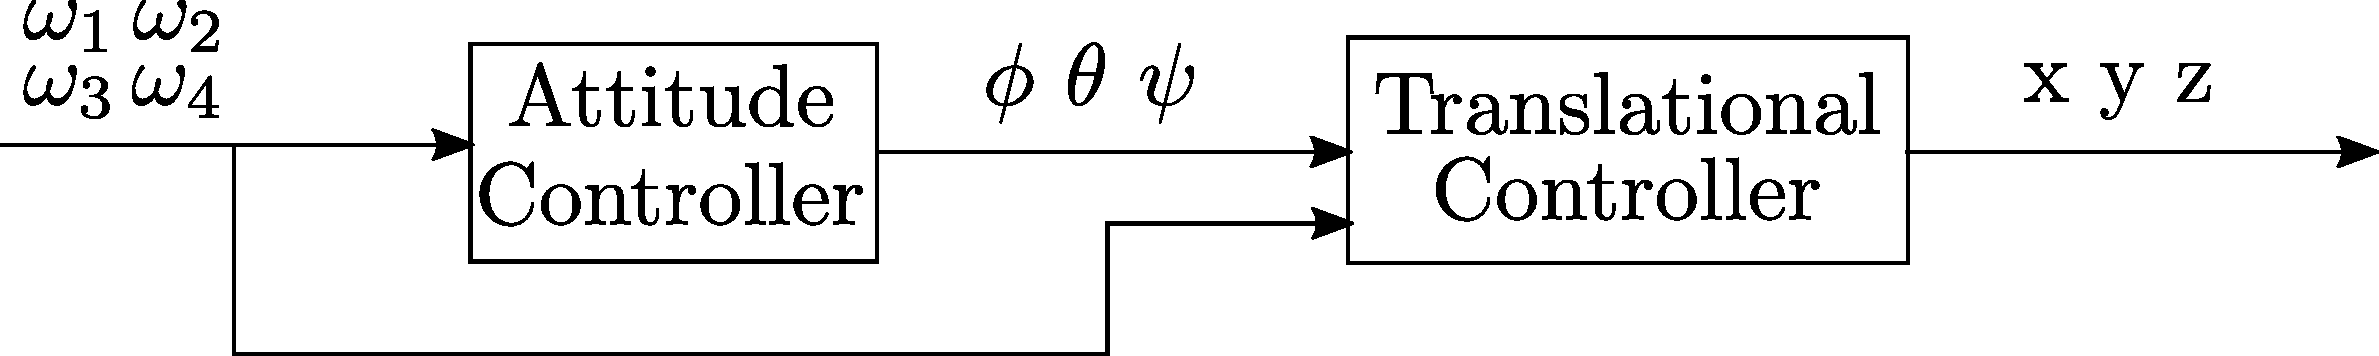
\includegraphics[scale=0.3]{figures/modelOverview}
    \caption{Overview of how the two models are related.}
    \label{fig:modelOverview}
\end{figure}
\vspace{-0.7 cm}
\autoref{fig:modelOverview} shows the relation between the two submodels. The attitude model, which describes the angular behavior, takes the velocities of the four motors as input and provides the angles roll, pitch and yaw as output. The translational model takes the angles as input, which also takes the rotational speeds of the motors as input. The output of the translational model is a position given in x, y and z coordinates.

When flying a quadcopter two different configurations are generally considered, the cross and the plus configurations, see \autoref{fig:plusConfiguration} and \ref{fig:crossConfiguration}. The angles of rotation, roll, pitch and yaw, are generally defined around the three coordinate axes attached to the quadcopter. \cite{HLChan}
\vspace{-0.6 cm}
\begin{figure}[H]
  \centering
  \captionbox
  {
    The quadcopter with orientation in the coordinate system corresponding to plus configuration.
    \label{fig:plusConfiguration}
  }
  {
    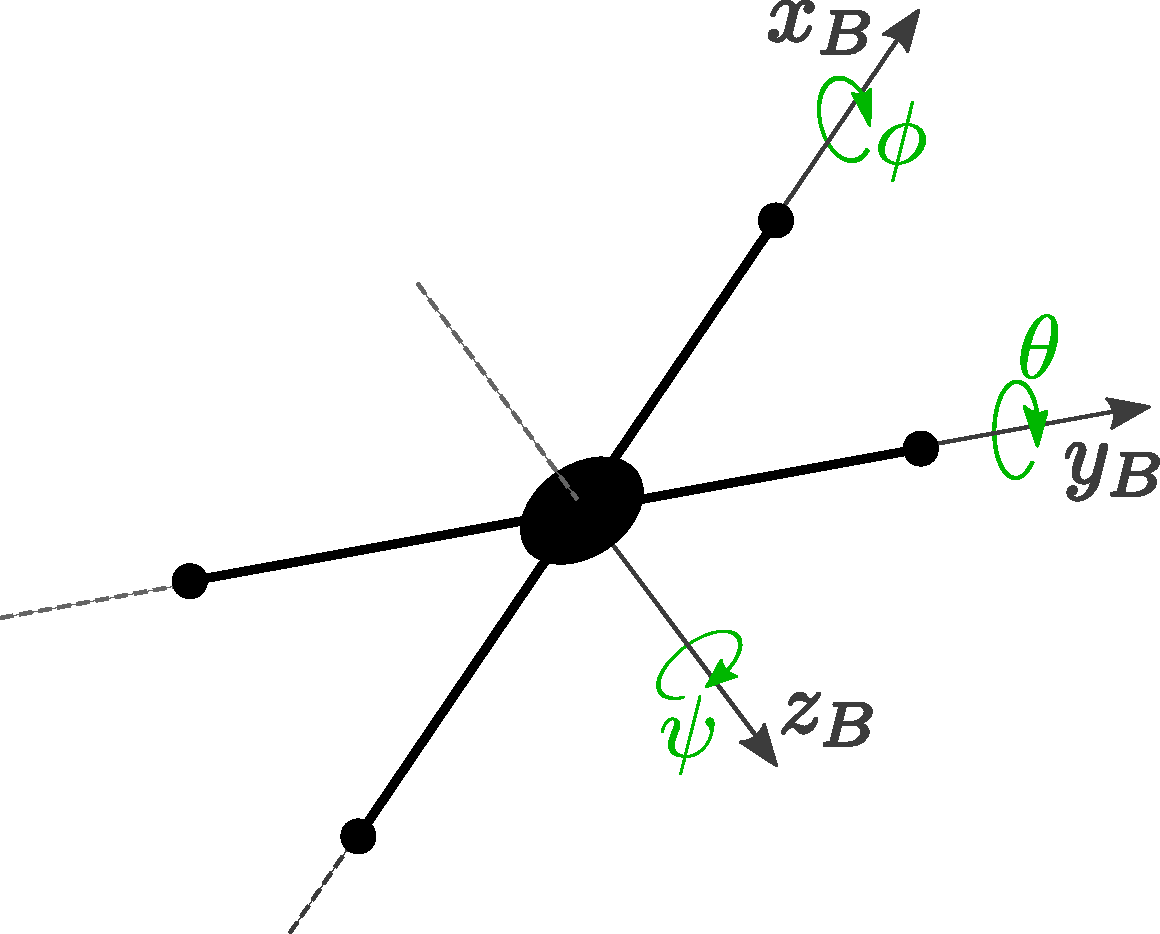
\includegraphics[width=.40\textwidth]{figures/plusConfiguration}
  }
  \hspace{5pt}
  \captionbox
  {
    The quadcopter with orientation in the coordinate system corresponding to cross configuration.
    \label{fig:crossConfiguration}
  }
  {
    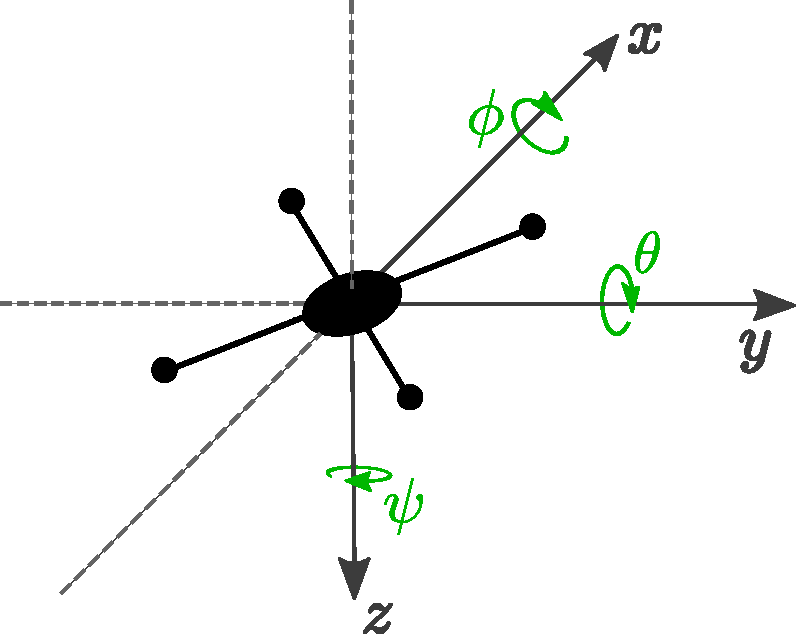
\includegraphics[width=.40\textwidth]{figures/crossConfiguration}
  }
\end{figure}
If the quadcopter is in plus configuration and i.e. the roll angle is increased, it will fly with one rotor in front. However if the same angle is applied to a quadcopter in cross configuration, it will fly with two rotors in front. \cite{HLChan}

Cross configuration provides a more responsive flight since all four rotors are engaged when changing an angle. Less actuation is also required from each motor since there are two to pull the quadcopter around. From a control perspective it is however more forthright to model and control a quadcopter in plus configuration, which is the choice for this prototype. \cite{HLChan}

An aspect to be mentioned before modeling the quadcopter is the usage of two coordinate frames. A body frame, which is fixed to the flying object, and an inertial frame, which is fixed to the Vicon room. 
%
\begin{figure}[H]
    \centering
    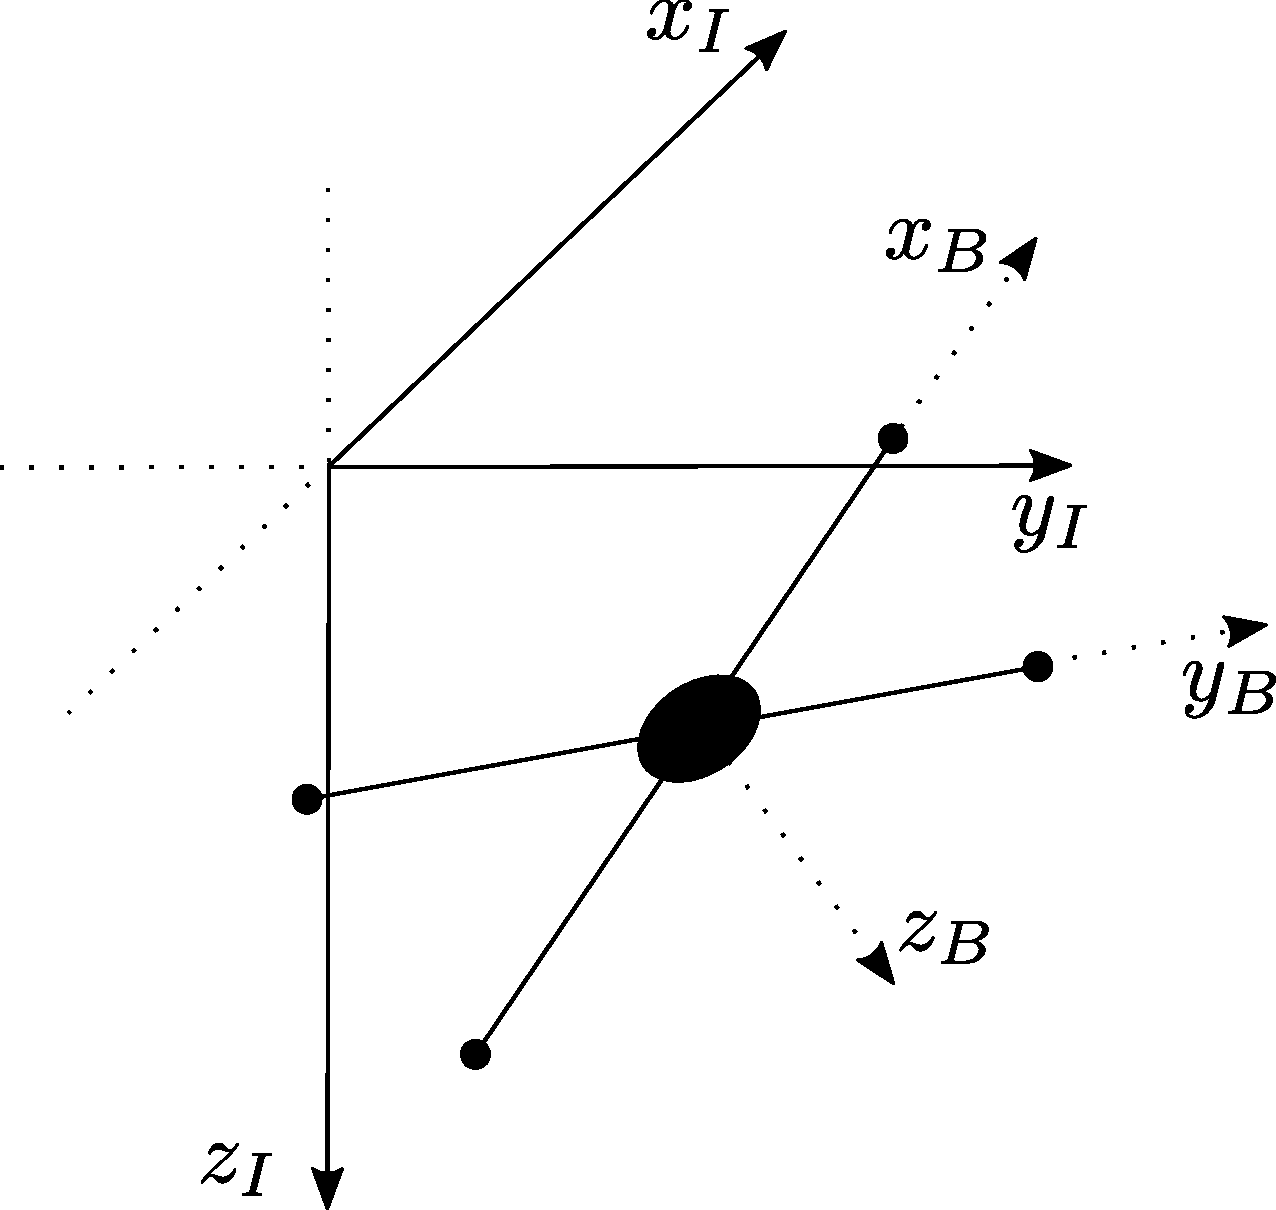
\includegraphics[scale=0.3]{figures/framesDiagram}
    \caption{The quadcopter with its body frame (B-index) placed in the intial frame (I-index) of the Vicon room. }
    \label{fig:framesDiagram}
\end{figure}

\autoref{fig:framesDiagram} shows the two frames. The inertial frame is oriented in such a way that its z-axis is pointing downwards, where altitude is given in negative numbers and ground is zero.

The attitude of the quadcopter is obtained by knowing the body frame orientation with respect to the inertial frame, yielding the roll, pitch and yaw angles. 

The transformation from the body frame to the inertial can be done through a rotation matrix, \autoref{eq:RotMatrix}, which describes a total rotation in terms of three consecutive rotations. \newpage
In this case the rotation matrix is composed with a 1-2-3 convention, that is, first a rotation around $x_{\mathrm{B}}$, then around $y_{\mathrm{B}}$ and finally around $z_{\mathrm{B}}$. \cite{rotationmatrix}

\begin{minipage}{0.32\linewidth}
    \begin{flalign}
        \si{R_X} &=
        \begin{bmatrix}
            1 & 0        & 0         \\ 
            0 & c\phi  & -s\phi  \\ 
            0 & s\phi  & c\phi   \nonumber  
        \end{bmatrix} 	\label{eq:RotMatrix1}
    \end{flalign}
\end{minipage}\hfill
\begin{minipage}{0.32\linewidth}
    \begin{flalign}
        \si{R_Y} &=
        \begin{bmatrix}
            c\theta  & 0  & s\theta  \\ 
            0          & 1  & 0          \\ 
            -s\theta & 0  & c\theta  \nonumber 
        \end{bmatrix} 	\label{eq:RotMatrix2}
    \end{flalign}
\end{minipage}\hfill
\begin{minipage}{0.32\linewidth}
    \begin{flalign}
        \si{R_Z} &=
        \begin{bmatrix}
            c\psi & -s\psi  & 0  \\ 
            s\psi & c\psi   & 0  \\ 
            0       & 0         & 1  \nonumber 
        \end{bmatrix} 	\label{eq:RotMatrix3}
    \end{flalign}
\end{minipage}\hfill
\small
\begin{flalign}
	R = R_Z R_Y R_X =
	\begin{bmatrix}
		c\theta c\psi  & s\phi s\theta c\psi -c\phi s\psi  & c\phi s\theta c\psi + s\phi s\psi  \\ 
		s\phi c\theta  & s\phi s\theta s\psi + c\phi c\psi & c\phi s\theta s\psi - s\phi c\psi  \\ 
		-s\theta         & s\phi c\theta                           & c\phi c\theta
	\end{bmatrix} 	\label{eq:RotMatrix}
\end{flalign}
\normalsize
%
\begin{where}
\va{R_X}{is the matrix describing a rotation around the $x_\mathrm{B}$ axis}{}
\va{R_Y}{is the matrix describing a rotation around the $y_\mathrm{B}$ axis}{}
\va{R_Z}{is the matrix describing a rotation around the $z_\mathrm{B}$ axis}{}
\va{R}{is the total rotation matrix}{}
\va{\phi}{is the roll angle}{rad}
\va{\theta}{is the pitch angle}{rad}
\va{\psi}{is the yaw angle}{rad}
\end{where}

Note that due to the size of the matrix sine and cosine are denoted $s$ and $c$ respectively.

To describe a vector in the inertial frame given its description in the body frame, a matrix-vector multiplication can be done as follows:
\begin{flalign}
    v_{\mathrm{I}}=Rv_\mathrm{B} 
\end{flalign}
\begin{where}
    \va{v_{\mathrm{I}}}{is a column vector that contains the description with respect to the inertial frame}{}
    \va{v_{\mathrm{B}}}{is a column vector that contains the description with respect to the body frame}{}
\end{where}

Once these considerations have been taken into account, the two submodels can be derived.

%Angle and Linear
%Explain the two frames and include drawing showing them
%Flow of the chapter

%\Figref{diagramQuad} shows a representation of the quadcopter where two reference systems, inertial and body, can be seen, as well as the conventions for angles of rotation and forces. \Figref{diagramTorque} shows the body from above and includes the chosen convention for the torques produced by the propellers.
%
%\begin{minipage}{\linewidth}
%	\begin{minipage}{0.45\linewidth}
%		\begin{figure}[H]
%			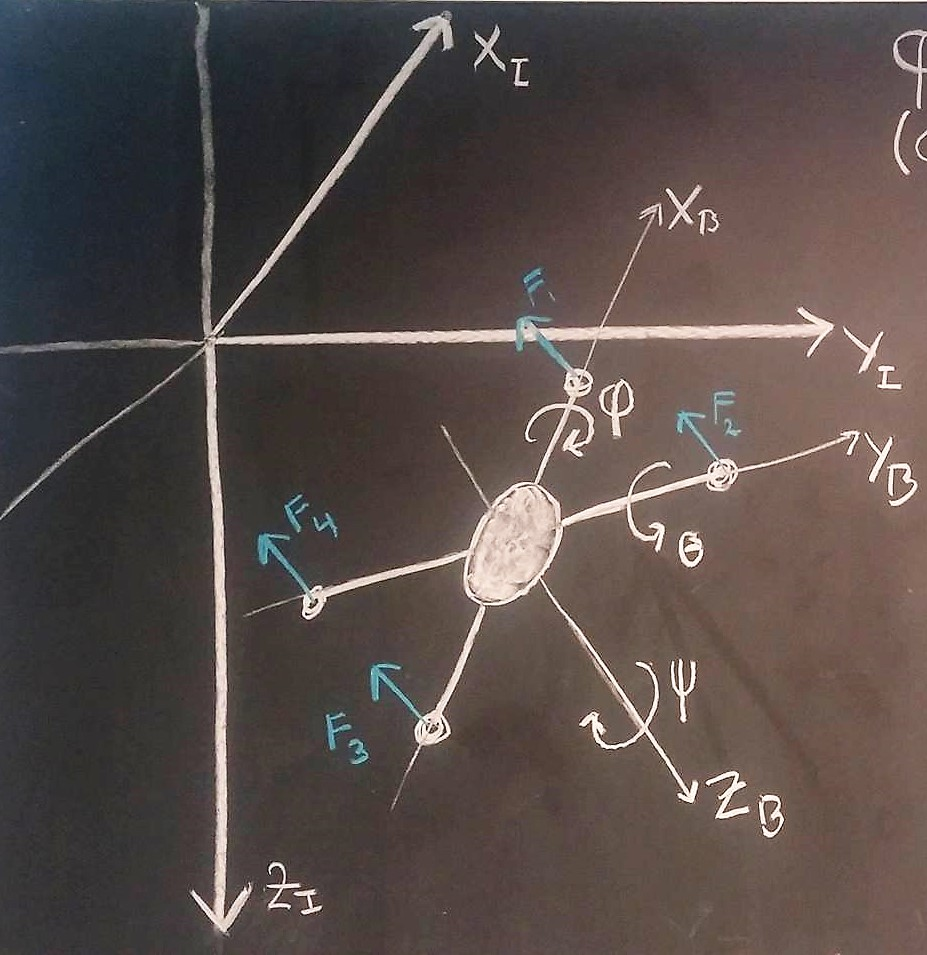
\includegraphics[scale=.27]{figures/drone_diagram}
%			\centering
%			\captionsetup{justification=centering}
%			\captionof{figure}{Diagram of the quadcopter which includes inertial and body reference systems, as well as the references for the angles (roll, pitch and yaw and the thrust forces produced by the propeller. }
%			\label{diagramQuad}
%		\end{figure}
%	\end{minipage}
%	\hspace{0.03\linewidth}
%	\begin{minipage}{0.45\linewidth}
%		\begin{figure}[H] \vspace{16mm}
%			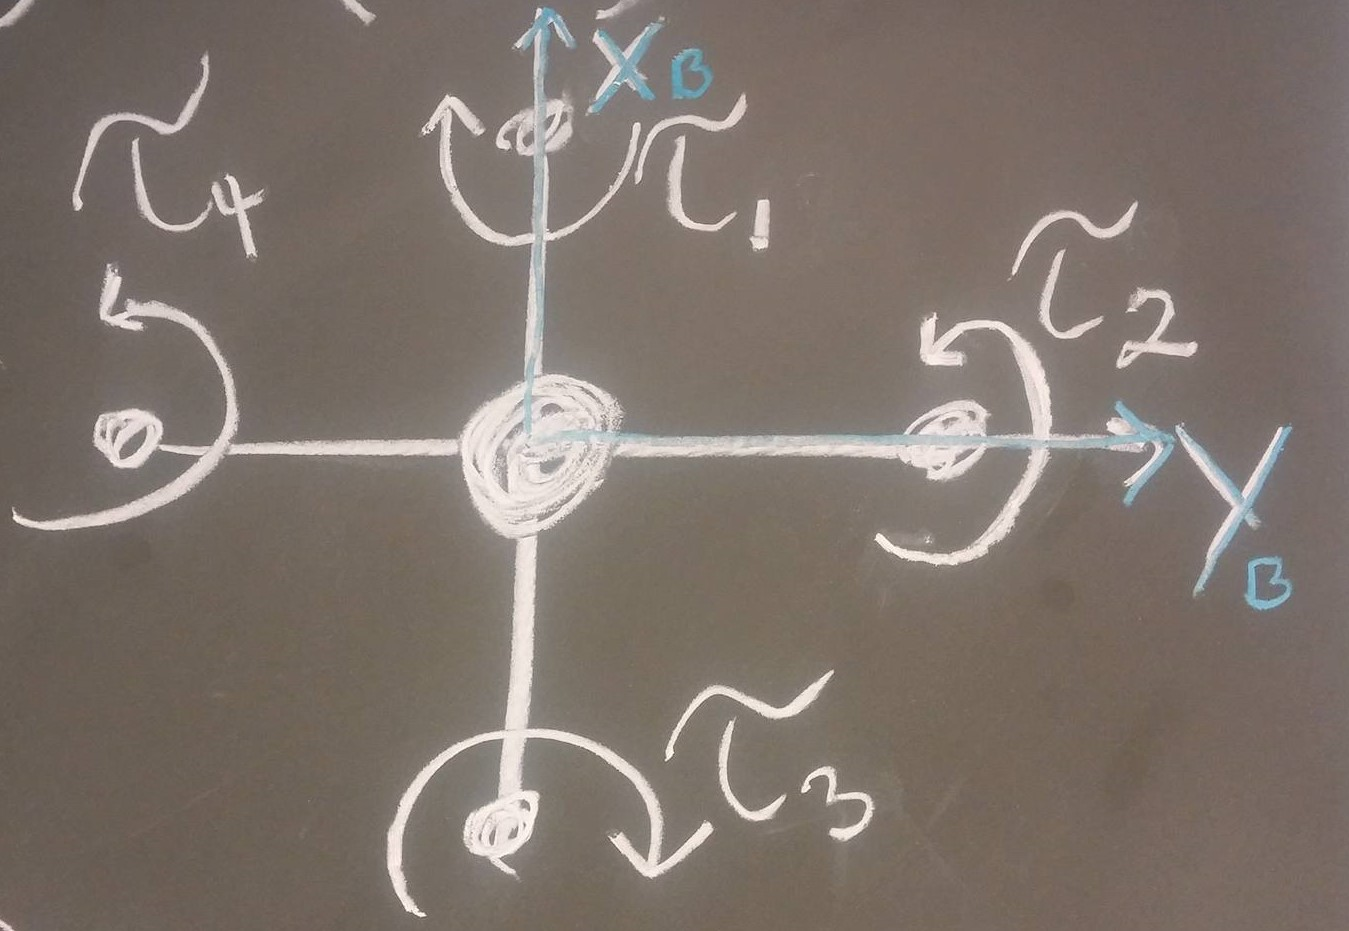
\includegraphics[scale=.18]{figures/torques_diagram}
%			\centering
%			\captionsetup{justification=centering}
%			\captionof{figure}{Diagram of the quadcopter from above, with the references for the torques produced by the drag force at the propeller.}
%			\label{diagramTorque}
%		\end{figure}
%	\end{minipage}
%\end{minipage}
%In the following section the attitude model is derived. 
\newpage